% The use of phonetic motor invariants can improve automatic phoneme discrimination
% Castellini, Metta, Fadiga, Badino
% submitted to PNAS

\documentclass{pnastwo}

% ---------------------------------- bookkeeping

% remove for submission
\usepackage[dvips]{graphicx}

%\usepackage{pnastwoF}
\usepackage{amssymb}
\usepackage{amsfonts}
\usepackage{amsmath}

\newcommand{\lio}{\textsf{lio}}
\newcommand{\ttu}{\textsf{ttu}}
\newcommand{\vlio}{\textsf{vlio}}
\newcommand{\vttu}{\textsf{vttu}}
\newcommand{\alio}{\textsf{alio}}
\newcommand{\attu}{\textsf{attu}}

\newcommand{\overall}{\emph{overall}}
\newcommand{\spka}{\emph{spk5vs1}}
\newcommand{\spkb}{\emph{spk3vs3}}
\newcommand{\spkc}{\emph{spk1vs5}}
\newcommand{\coa}{\emph{coart4vs1}}
\newcommand{\cob}{\emph{coart3vs2}}

%%%%%%%%%%%%%%%%%%%%%%%%%%%%%%
%% Don't type in anything in the following section:
%%%%%%%%%%%%
%% For PNAS Only:
\contributor{Submitted to Proceedings
of the National Academy of Sciences of the United States of America}
\url{www.pnas.org/cgi/doi/10.1073/pnas.0709640104}
\copyrightyear{2008}
\issuedate{Issue Date}
\volume{Volume}
\issuenumber{Issue Number}
%%%%%%%%%%%%

\begin{document}

% ---------------------------------- frontmatter

\title{The use of phonetic motor invariants\\
can improve automatic phoneme discrimination}

\author{
Claudio Castellini\affil{1}{LIRA-Lab, University of Genova, Italy},
%\affil{6}{Now at the German Aerospace Research Center, Oberpfaffenhofen, Germany},
Leonardo Badino\affil{2}{Italian Institute of Technology, Genova, Italy},
Giorgio Metta\affil{1}{}\affil{2}{},
Giulio Sandini\affil{1}{}\affil{2}{},
Michele Tavella\affil{1}{},
Mirko Grimaldi\affil{5}{CRIL, Salento University, Italy} and
Luciano Fadiga\affil{4}{DSBTA, University of Ferrara, Italy}
}

\contributor{Submitted to Proceedings of the National Academy of Sciences
of the United States of America}

\maketitle

\begin{article}

\begin{abstract}

  We hereby investigate the use of phonetic motor invariants (MIs),
  that is, recurring kinematic patterns of the human phonetic articulators,
  to improve automatic phoneme discrimination. Using a multi-subject
  database of synchronized speech and lips/tongue trajectories, we first
  identify MIs commonly associated with bilabial and dental consonants,
  and use them to simultaneously segment speech and motor signals.
  We then build a simple neural network-based regression schema (an Audio-Motor
  Map, AMM) mapping audio features of these segments to the corresponding
  MIs.
  
  Extensive experimental results show that
  $(a)$ a small set of features extracted from the MIs, as originally gathered from
    articulatory sensors, are dramatically more effective than a large, state-of-the-art
    set of audio features, in automatically discriminating bilabials from dentals;
  $(b)$ the same features, extracted from AMM-reconstructed MIs, are as effective as
  or better than the audio features, when testing across speakers and coarticulating phonemes;
    and dramatically better as noise is added to the speech signal.
  
  These results support some of the claims of the motor theory of speech perception
  and add experimental evidence of the actual usefulness of MIs in the more general
  framework of automated speech recognition.
  
\end{abstract}

\keywords{motor theory of speech | machine learning | phoneme discrimination | speech recognition}

% ---------------------------------- the paper

\section{Introduction/Motivation}
\label{sec:intro}

\dropcap{A}utomatic speech recognition (ASR) is the ability of a machine
to convert human speech, coded as an audio signal, into words.
Potential applications of ASR range from human-computer interfaces
to informatics for the disabled to data mining in large speech corpora.
Despite decades of research, state-of-the-art ASR
systems still need to be trained upon very large and heterogeneous data sets
to account for speech variability.
%, or upon a single speaker's speech in controlled conditions.
And nevertheless, human beings show an excellent ability
of understanding one another's speech, independently of the speaker, the
accent, the pitch and speed, noise, etc.

Recent neuroscientific
evidence indicates that the brain motor areas responsible for producing labial
and dental phonemes are also involved in their perception; D'Ausilio et al. \cite{dausilio}
show that in a discrimination task of /b/,/p/,/d/ and /t/, trans-cranial magnetic
stimulation of the lips and tongue \emph{motor areas} creates a bias in favor
of the \emph{perception} of labials, and similarly, stimulation of the tongue
favors dentals. This suggests that motor information may be paramount for
understanding speech in humans.

Inspired by these finding, in this paper we investigate whether the knowledge of speech production in humans 
integrated into an automatic phoneme classifier improves the identification in the acoustic dimension 
of the specific behaviors of the /b/,/p/,/d/ and /t/ plosive consonants.
 
In ASR, approaches that combine explicit speech production knowledge and audio features
have been proposed (see \cite{king} for a review) as alternatives 
to the classic approach  in which the complex acoustic effects of speech production variability 
(e.g., due to speaking rate) and coarticulation (the phenomenon by which the phonetic realization of a phoneme is affected by its phonemic context) are directly and implicitly modeled in the acoustic domain.

%Although conclusions on the actual utility of speech production knowledge are somehow contradictory

By limiting our investigation on the utility of motor information to the much simpler (than ASR) task of four consonants classification\footnote{Note that a recognition task requires both segmentation of speech into phones and their classification.} we are able to relax working assumptions and avoid technical difficulties that so far have hampered a satisfactory integration of motor information into ASR systems. 

Additionally, from previous work it is not feasible to properly identify which aspects of the recognition process benefit from motor information. For example, motor knowledge may improve the modeling (and so the identification) of coarticulation effects that are seen in the training data set, but not necessarily improve the recognition of phonemes in unseen contexts, i.e., it may not necessarily improve the generalization ability of the ASR system. On the other hand the experimental setup we have designed has the main goal of investigating whether motor information improves the generalization ability of a phoneme classifier.  

%Although the integration of speech production knowledge in an ASR system often brings some improvements, %it is commonly held that the potential of speech production knowledge is far from being exhaustively exploited.  

To this end, we have focused on the automatic version of
the problem tackled in D'Ausilio et al.'s work. For each consonant,
a corresponding typical phonetic motor invariant (MI) was
identified according to basic physiology of speech;
e.g., a fast, voiced opening (plosion) of the lips for /b/, and so on.
MIs were then used to semi-automatically segment the audio/motor data found in a
database of speech/motor trajectories recorded from $6$ subjects.

Subsequently, a simple regression method (namely, a feed-forward neural network) was employed
to build an Audio-Motor Map (AMM), which converts audio features of the isolated segment to
features of the related MI. On an abstract level, an AMM is a mathematical proxy of a mirror
structure \cite{umilta-01}, reconstructing the distal speaker's speech production act while
listening to the related piece of speech.

To test the approach, we have devised three experiments involving a 
classifier in the form of a Support Vector Machine \cite{BGV92}. We wanted to check whether
the use of MI-based features, either those recorded in the database (the ``real''
motor features) or the AMM-reconstructed ones (a more ecological scenario),
could improve the classifier's performance. Our results show that this is the case,
especially when the classifier is trained on incomplete data sets such as 
per-speaker (e.g., training on speakers $1,2,3$ and testing on $4$) and
per-coarticulation(e.g., training on /ba/, /be/, /bi/, /bo/ and testing on /bu/); or when noise is added,
in which case motor features significantly help classification, even when added to a
state-of-the-art set of audio features about $20$ times larger than that extracted
from the MIs.

\subsection{Related Work}

It is known since the Sixties \cite{liberman1} that the audio signal of speech
cannot be effectively segmented down to the level of the single phoneme,
especially as far as stop consonants such as bilabial plosives
are concerned; in particular, their representations in the audio domain are
radically different according to the phoneme which immediately follows.
It remains an open question then, how humans can
distinctly perceive a common phoneme, e.g.,/b/ in  /ba/ and /bi/, since they
apparently have access to the speaker's audio signal only.

The explanation put forward by the so-called motor theory of speech perception
(MTS, \cite{liberman2,galant}) is that, while perceiving sounds,
humans reconstruct \emph{phonetic gestures}, the physical acts of
producing the phonemes, as they were trained since birth to associate
articulatory gestures to the sounds they heard. 

Even ignoring the motor theory of speech perception the use of speech production knowledge is appealing in that the coupling of articulatory and audio streams allows for explicit models of the effects of speech production phenomena (e.g., coarticulation) on the acoustic domain. These effects cannot be precisely modeled (e.g., when the phoneme /a/ affects the phonetic realization of /b/ in /ba/?)  or modeled at all (e.g., what happens when I utter a /o/ with exaggeratedly open jaw?) when the phonemic stream is directly mapped onto the acoustic dimension as in the standard approach to ASR.  

Different solutions have been proposed to integrate speech production knowledge into an ASR system and different types of speech production information has been used, ranging from articulatory measurements (see \cite{zlokarnik,stephenson,wrench}, for example) to symbolic non-measured representations of articulatory gestures that "replicate" a (symbolic) phoneme into all its possible articulatory configurations\footnote{Articulatory configurations are configurations of the positions of the phonetic articulators} (see \cite{richardson, livescu}, for example).
 
   
%One possible reason why ASR is so difficult is then that
%machines have in general no access to the motor representation of the
%audio signal they are supposed to understand. We hypothesize that motor 
%information might help ASR, especially when tests on different speakers and different
%coarticulations are performed: for example, when training on subject $A$ and
%testing on subject $B$, or when training on pseudo-words such as /ba/, /bi/,
%/be/ and then testing for the presence of /b/ in /bo/, /bu/ or even /br/.

Although some studies have shown increased word recognition accuracy when including speech production knowledge in ASR, it is commonly held that the potential of speech production knowledge is far from being exhaustively exploited. Limits of current approaches include: the use of the phoneme as basic unit (as opposed to articulatory configuration, for example) which appears to be too "coarse", especially in the context of spontaneous spoken speech 
%where coarticulation effects are more frequent and marked
;and  the lack of a mechanism that accounts for the different importance of articulators in the realization of a given phoneme (e.g., in the generation of phoneme /b/ lips are critical, i.e., important, while tongue is non-critical).

The traditional approach in which the speech signal is segmented into phones, often referred to as "beads on a string" approach, poses problems to an accurate modeling of spontaneous speech where coarticulation phenomena such as phone deletion or assimilation (where a phone assimilates some articulatory gestures of the preceding/following phone), are frequent and not always predictable and call for finer-grained basic units (see \cite{ostendorf})). To partly make-up for such limitation we propose an alternative approach where, instead of segmenting the audio stream looking at audio features only and then observing the articulatory gestures within the identified phones, we give priority to the motor information in that speech is segmented by searching for phone-specific patterns of the (critical) articulatory gestures.

%Concerning the necessity of a phoneme dependent distinction between critical and non-critical articulators we do not 
%Traditionally (e.g., \cite{bourl,salvi}), the audio speech signal is segmented with a
%fixed-length Hamming window, usually 20ms. long. The resulting sequence
%is then analysed in the frequency or cepstral domain and the
%resulting coefficients are used as features for a classification system.
%One negative aspect of this approach is that it
%neglects the qualitative overall characteristics of the
%phoneme being uttered: depending on the speed of the speech, a consonant
%can have different lengths and, by using the above approach, global
%information about it is lost (see \cite{ostendorf}, where this approach is
%dubbed ``beads-on-a-string''). Nevertheless, as far as we know, there is
%so far no widely accepted alternative method for speech segmentation,
%if the audio signal is the only one available. One attempt, but not based
%upon articulatory data atl all, appears in \cite{bourlard}.


During recognition, articulatory gestures have to be recovered 
from audio information as audio is the only signal available.
Reconstruction of articulatory features has been attempted since a long
time, but in most cases it is not derived from articulatory \emph{data}
gathered from human subjects. One pioneeristic case is that of Papcun
et al. \cite{papcun} where the AMM is carried out by a Multilayer Perceptron.
Our procedure for building the AMM is deeply inspired by this work.
%By using a Multilayer Perceptron we implicitly assume that all articulators have the same importance and that the AMM is a %one-to-one mapping.   
%Papcun et al. \cite{papcun} observed that non-critical articulators have higher variance (in terms of position) than critical %articulators. 
The Multilayer Perceptron tries to carry out the best recovery of all articulatory gestures while more emphasis to the recovery of the gestures of the critical articulators should be given to the detriment of the non-critical articulators, which have higher variance (in terms of position, see \cite{papcun,rose}). Although we do not address this issue, the simple fact that we only consider two articulators alleviates a problem that would be otherwise far more relevant if all articulators were taken into account\footnote{The higher variance of the non-critical articulators is the main cause that makes AMM a one-to-many mapping: different articulatory configurations result in the same acoustic realization. Solutions to properly address this "ill-posed" nature of the AMM have been proposed by Richmond et al. \cite{richmond} and Toda et al. \cite{toda}. }.

%and subsequently Korin Richmond's work
%\cite{richmond2002,richmond2007} who have been able to reconstruct point-by-point
%the trajectories of articulators from the audio signal to a remarkably low
%error rate. The procedure for building the AMM is deeply inspired by their
%work.

Interestingly, the idea of using information about the mechanisms involved in the production of a human action to improve its classification/recognition (in a domain different from the production domain) has not only been applied in the context of speech recognition. For example Metta et al. \cite{metta-06} and Hinton \cite{hinton-2006} 
have shown that articulatory data can improve classification accuracy in automated hand action classification.

%TODO  
% Transferring the method to speech perception seems
% like a natural choice.

\section{Data Set}
\label{sec:dataset}

\subsection{Subjects and Set-up}
\label{subsec:setup}

Six female Italian native speakers were recorded while uttering
Italian words and pseudo-words. Words were mainly stress-initial, e.g.,
"matto", "nome", "strada" (mad, name, road), and were chosen in order
to have consonants both at the beginning and in the middle of
words, followed by different vowels and consonants.
The data recording setup included a \emph{Laryngograph Microprocessor}
device (Laryngograph Ltd., London, www.laryngograph.com) which gathers speech audio
signal and the electroglottographic (EGG) signal at $16$KHz sampling
rate; and an AG500 electromagnetic articulograph (Carstens Medizinelektronik
GmbH, Germany, www.articulograph.de) that records the
3D positions of a set of sensors glued on the tongue, lips and front teeth
during speech production at a sampling rate of $200$Hz. A full description of the 
acquisition set-up and the obtained database can be found in \cite{tavella}.

The subset used in this work comprises the $77$ words in the database
which contain /b/, /p/, /d/ or /t/. This includes utterings from each of the
$6$ subjects; consonants are found both at the beginning of the word or
in the middle; and they are followed by either /a/,/e/,/i/,/o/,/u/,/r/ or /s/.
From now on, the phoneme appearing immediately after a consonant will be called
\emph{coarticulating} phoneme.

\subsection{MI-Based Signal Segmentation}
\label{subsec:segm}

We define the length of a phoneme in terms of the MI underlying its production;
the audio signal is, therefore, segmented according to it.
A qualitative examination of the synchronised audio and motor
signals obtained from utterances of /b/, /p/, /d/ and /t/
by different speakers indicates that common patterns can
actually be found in the behaviour of the related articulators.
For instance, as is apparent from Figure \ref{fig:isdView}, 
recurring shapes of the lips opening velocity and acceleration appear
when both /ba/ and /bufalo/ are considered, even when uttered by different
speakers. The same patterns can be observed and are qualitatively clear when other
words containing /b/ and /p/ are considered, both when the phoneme appears at the
beginning or inside a word, and regardless of the coarticulating phoneme.

These observations visually confirm the basic taxonomy of stop consonants 
as found in any linguistics textbook. In particular, all considered consonants are plosives,
i.e., consonants that involve a complete blockage of the oral cavity followed by a fast
release of air. /b/ and /p/ are bilabials (blockage produced using the upper and lower lips)
while /d/ and /t/ are dentals (blockage produced using the tongue tip and the upper teeth).
The following motor invariants are then defined and associated to the consonants under
examination:

\begin{itemize}

  \item Let $s_1(t)$ and $s_2(t)$ be the signals associated
    with sensors placed on two phonetic actuators (e.g., the upper and
    lower lips), and $\delta(t) = ||s_1(t)-s_2(t)||$ be their
    Euclidean distance. Then, a plosion is defined as the interval
    between two instants $t_{start}$ and $t_{end}$ such that
    $\dot{\delta}(t_{start}) = 0 $ and $\ddot{\delta}(t_{start}) > 0$,
    and $\dot{\delta}(t_{end}) > 0 $ and $\ddot{\delta}(t_{end}) = 0$.

  \item For /b/ and /p/, the sensors on the upper and lower
    lip are considered for $s_1(t)$ and $s_2(t)$, whereas for /d/ and /t/
    those on the tongue tip and upper teeth are. In turn, the associated
    distances will be denoted as \lio\ (lips opening) and \ttu\
    (tongue tip - upper teeth distance). As well, the respective velocities
    and accelerations will be denoted by \vlio, \vttu, \alio, \attu.

\end{itemize}

The first condition physically defines a plosion, e.g., considering \lio, $t_{start}$
marks the onset of the act of opening the lips (null velocity, positive acceleration)
while $t_{end}$ is found at the instant of maximum opening velocity and zero acceleration.
The choice of cutting the signals at $t_{end}$ rather than, say, when the lips are still
and \lio\ is maximum is motivated by the need to capture the plosion only, with as little
as possible of the following phoneme. By manual (audio) inspection of the audio segments so
obtained, we could actually verify that only a tiny fraction of the coarticulating phoneme
could be heard at the end of the uttering.

The second condition then selects an appropriate pair of articulators needed for the
phoneme under consideration. This schema matches the above-mentioned taxonomy. In Figure
\ref{fig:isdView} the gray zone indicates the detected interval of time using conditions
$1$ and $2$. We expect that the same schema could be used to identify relevant MIs for
other consonants, e.g., an alveolar plosion for /k/ and /g/ and so on --- of course one
must have had the right sensors in place.

The segmentation is carried out semi-automatically: for each
utterance, all sequences matching the above conditions are displayed and the
associated speech is played, so that the experimenter can choose whether the
sequence is a correct guess or it is a false positive. In this experiment we only
monitor \lio\ and \ttu, so that false positives appear, e.g., when considering
/ts/ and /dz/. This is why, at this stage, a completely automatic segmentation
cannot be enforced. If the sequence is accepted, it is labelled
with the associated consonant, the speaker, and the
coarticulating phoneme. For example, from the word /bronzo/ (bronze) a /b/
sequence is extracted, and the letter "r" is stored as the coarticulating phoneme.
This way, from the original $77$ words and pseudowords, a total
of $1157$ audio/motor sequences are extracted, with a length of $122 \pm 41.2$
milliseconds (mean $\pm$ one standard deviation).

% qui potremmo mettere una tabella con le statistiche sul data set:
%
%In turn, 
%
%\begin{itemize}
%
%  \item $292$ /b/, $303$ /p/, $59$ /d/ and $503$ /t/;
%
%  \item $213,149,156,229,241,169$ for subjects $1,\ldots,6$;
%
%  \item $352,59,99,377,167,71,32$ for each coarticulating phoneme
%    /a/, /e/, /i/, /o/, /u/, /r/ and /s/.
%
%\end{itemize}
%
%Notice that no distinction is made whether the consonant is at the beginning
%of an utterance (e.g., /b/ in /baffo/, moustache) or in the middle of
%it (e.g., /d/ in /strada/, \emph{road}).

\subsection{Cross-validation}
\label{subsec:cv}

As is standard practice in machine learning, the obtained dataset was divided into
splits to perform cross-validation (CV). CV \cite{stat} is usually used
to estimate the generalisation error of a learning machine, at the
same time providing a ground for grid-searching the optimal parameters\footnote{These
two points should really be independent of each other, a feature provided, e.g., by
\emph{nested} CV \cite{nestedCV}; but here the size of the dataset is
prohibitively small for such an analysis.}. The dataset was therefore divided into
$10$ equally sized random disjoint sets, whose union coincides with the original dataset; every
learning machine would then be trained upon $9$ of these sets and tested upon the
tenth. This ensures that no data used for testing have been used for training. Such a
training/testing set pair is called a \emph{split}. (Testing data are normalised using the
statistics of the training set.) After choosing a standard performance index for the machine
considered (e.g., the balanced error rate for classifiers), we would run the machine
on each split and show the mean performance, plus/minus one standard error of the mean,
that is the standard deviation divided by the square root of the number of splits.

We will call this type of CV, the \emph{overall} CV schema,
since every training and testing set contains data tagged with every subject and
coarticulating phoneme. In our case, however, CV is also used to perform more subtle
tests, for instance to check whether a classifier trained on some subjects would
then effectively predict samples uttered by an another subject; or whether a classifier
trained upon a subset of coarticulating phonemes (e.g., on /$\alpha\beta$/ with
$\alpha \in \{b,p,d,t\}$ and $\beta \in \{a,e,i,o\}$) would then effectively predict samples
coarticulated with other phonemes (in the example above, predict samples of the form
/$\alpha\gamma$/ with $\gamma \in \{u,r,s\}$). To this end, $5$ more CV schemas were devised:

\begin{itemize}

  \item \spka\ The training sets contain samples
  	uttered by $5$ speakers while the testing set is
  	uttered by the remaining speaker; this gives us $6$ splits.

  \item \spkb\ Likewise, but training on $3$ speakers and testing on the
  	other $3$. This results in $\binom{3}{6} = 20$ splits.

  \item \spkc\ Likewise, but training on $1$ speaker and testing on the
  	other $5$, resulting in $6$ splits.

  \item \coa\ The training sets contain samples
  	with $4$ coarticulating vowels, whereas the testing sets contain samples
  	with the remaining two, plus /r/ and /s/. This gives us $5$ splits.

  \item \cob\ Likewise, but training on $3$ coarticulating vowels and
  	testing on the remaining $2$ plus /r/ and /s/. This gives us
  	$\binom{3}{5} = 10$ splits.

\end{itemize}

Notice that, the more splits, the more reliable the results are, as far as the
generalisation error is concerned; but as well, in some cases the training sets
are rather small if compared to the testing sets. This is the reason why we could
not try, e.g., a CV schema with training on utterances containing
one coarticulating vowel and testing on all the others (e.g., training on
/$\alpha$a/ and testing on /$\alpha\beta$/, where $\alpha$ is any consonant
and $\beta \in \{e,i,o,u,r,s\}$.

\section{The Audio-Motor-Map}
\label{sec:rec}

\subsection{Training the AMM}
\label{subsec:amm_setup}

The procedure for building the AMM closely follows that outlined in
\cite{papcun,richmond2002,richmond2007} for a multi-layer perceptron.
For each of the $1157$ audio sequences, the spectrogram is evaluated
over time windows (slices) of $20$ milliseconds, using a $20$ filter
Mel-scale filterbank between $20$Hz and $2$KHz.
Each slice overlaps by $10$ milliseconds with
the preceding slice. Then point by point, the velocity and acceleration of
\lio\ and \ttu\ (from now on, in turn, \vlio, \alio, \vttu\ and \attu) are
associated to $19$ spectrogram slices, covering about $200$ milliseconds
of speech and centered around the point itself.
%Figure \ref{fig:amm} graphically represents the procedure.

This way, about $15000$ samples are extracted from the original $1157$
audio/motor sequences; each input sample consists of $19\cdot 20 = 380$ real
numbers, while the output space is given by the $4$ trajectory points of
the motor signals. A feed-forward neural network is set up in order to
build the AMM, with $380$ input units, one hidden layer with $15$ units and
$4$ output units; the net is trained via the Scaled Conjugate Gradient
Descent method \cite{MOLLER93} and the activation is a logistic sigmoidal function.

Training is done via early stopping on the approriate validation set (see the previous
Section for the details about CV). This procedure is repeated over $10$ random restarts, and then
the network with best average performance over the $4$ output dimensions is stored.
%We have manually verified that all training sessions end by validation stopping
%(as opposed to bumping into the maximum number of training epochs, which we set
%for safety at a large value, $200$).
The performance measure is Matlab's embedded mean-square-error with regularisation
function, in which after some initial experiments we set the regularisation
parameter at $0.714$. This value, as well as all other parameters, have been found in
an initial experimentation phase, by slightly altering values suggested in literature
and/or in the Matlab manual.

Samples are normalised by subtracting the mean values
and dividing by the standard deviations, dimension-wise; targets are
normalised in order to lie within the range $[0.25,0.75]$, since the
logistic activation function has asymptotic values of $0$ and $1$.

\subsection{Evaluating the AMM}
\label{subsec:amm_results}

Figure \ref{fig:amm_perf} shows a quantitative assessment of the performance
of the AMM. The NRMSE ranges from $15.55\% \pm 1.11\%$ (\vlio, \coa ---
RMSE is normalised against the range of the signals considered) to
$8.07\% \pm 0.5\%$ (\vttu, \spkc). Regression upon \vlio\ shows the largest
errors, over all CV schemas.

Although these figures do not really indicate whether AMM-reconstructed MIs will be
effective in phoneme discrimination, they prove that the error rate in rergession has
limited magnitude and does not differ dramatically across CV schemas and output signals.
Qualitative inspection of the results (one example is given in Figure \ref{fig:example})
is encouraging, showing that the AMM-reconstructed motor signals are on average rather
similar to the real ones.

As a further test of reliability, we checked how good the performance is with respect
to what consonants are used as input, and what outputs are monitored. For each utterance,
the correlation coefficient between AMM-reconstructed and real MIs has been collected
according to whether labials (/b/,/p/) or dentals (/d/,/t/) had been presented as input
to the AMM.

As one can see in Figure \ref{fig:DD}, when the \overall\ CV schema is used,
there is a noticeable ``double dissociation''
pattern arising from the comparison of the correlation coefficients when the AMM
reconstructs \vlio\ and \vttu\ from labials or dentals. This pattern repeats to an
almost uniform extent when the other CV schemas are used.

\section{Phoneme discrimination}
\label{sec:class}

\subsection{Experiment 1}
\label{subsec:exp1}

In the first experiment the performance of a standard classifier is evaluated
according to the \overall\ CV schema for four different sets of features.
Figure \ref{fig:class1_perf} shows the results.

``Audio'' is a set of $20$ cepstral coefficients evaluated according to the
Mel scale over a bandwidth of $20$Hz to $2$KHz. This is a standard set of features
according to state-of-the-art literature, when the segment
length is fixed a priori. In this case the segment length is not fixed so the
cepstra are evaluated over the whole window, regardless of its length.

%
% Giorgio: qui il tempo viene buttato via?
%

``Real motor'' is a set of $17$ coefficients evaluated as follows: for each
signal considered (\vlio, \alio, \vttu\ and \attu), a least-squares cubic fit
is generated over the selected segment, that is, from $t_{start}$ to $t_{end}$
as defined above. This results in $4$ real numbers
per signal, which qualitatively encode the shape of the signal considered. The
$17$th number is the average of the voicing signal over the selected segment.

``Reconstructed motor'' refers to the same procedure as above, but applied
to the AMM-reconstructed signal curves.

Lastly, ``Joint'' denotes a decision procedure obtained by multiplying the
label probabilities obtained from the best classifiers for the audio and
reconstructed motor features.

The classifier is a Support Vector Machine \cite{BGV92} with Gaussian kernel
and hyperparameters $C, \sigma$ found by grid-search. Samples are normalised
by subtracting the mean values and dividing by the standard deviations,
dimension-wise.

The accuracies obtained are, in turn,
$87.64\% \pm 1.05\%$
$92.05\% \pm 0.70\%$
$87.38\% \pm 0.83\%$
$92.65\% \pm 1.00\%$, with statistically significant difference (Student's t-test,
$p<0.01$) between audio and real motor features, audio and joint features, and
reconstructed motor and joint features.

\subsection{Experiment 2}
\label{subsec:exp2}

Experiment 1 was replicated using this time the remaining CV schemas.
Figure \ref{fig:class2_perf} shows the results. (For comparison,
the Figure also shows in the first column the accuracies obtained for
experiment $1$.)

For each and every CV schema, the statistically significant differences seen in
Figure \ref{fig:class1_perf} are present (again, tested via $p$-values);
in particular, in the per-speaker CV schemas, the audio features versus
the joint models show accuracies of
$81.92\% \pm 2.04\%$ and $87.27\% \pm 1.17\%$ (\spka),
$78.90\% \pm 0.61\%$ and $85.74\% \pm 0.44\%$ (\spkb), and
$70.29\% \pm 0.73\%$ and $76.25\% \pm 1.53\%$ (\spkc).

In the per-coarticulation results the gap is more evident; the joint models
here perform worse than the reconstructed motor features. Audio features
versus reconstructed motor features show accuracies of
$41.60\% \pm 9.72\%$ and $62\% \pm 4.86\%$ (\coa) and
$34.84\% \pm 3.64\%$ and $55\% \pm 5.5\%$ (\cob).

\subsection{Experiment 3}
\label{subsec:exp3}

Lastly, for experiment 3 we replaced the audio features with
a $351$-dimensional set of $20$ mel-cepstral
coefficient, this time obtaining by taking $19$ slices of $20$ milliseconds each,
shifted over the audio segment by the required amount of time. This set of
features was compared, again, with the real and reconstructed motor features and
a probabilistic joint model, as white noise was added to the audio signals.

The intensity of noise was changed from nil to $150\%$ of the standard deviation
of each utterance considered; for each sample, $10$ noisy ones were generated, in
order to obtain a larger statistical basis. As in experiment $1$, the \overall\ CV
schema was chosen. Figure \ref{fig:class3_perf} shows the results.

(Notice that the real motor features are not affected by noise.) Student's t-test
reveals that the cepstra-2KHz and joint features are always significantly different.
The cepstra-2KHz and joint features show accuracies ranging from
$91.96\% \pm 0.22\%$ and $93.26\% \pm 0.25\%$ for no noise, to
$69.34\% \pm 0.47\%$ and $75.69\% \pm 0.53\%$ for maximum noise.

The results hereby presented clearly show that the plain, old EMG
signal can be used to drive a mechanical hand / prosthetic hand in a
radically new way: finer, force-controlling, more dexterous. Our
results indicate that a machine learning approach such as Support
Vector Machines will effectively detect well-separated grasping
patterns in real time, as required by an amputee; at the same time,
the system will be able to detect how much force is involved in the
grasp. If the prosthesis has a sufficient number of DOFs, that is, it
can be position-controlled to mimic the required grasps, and if it can
be force-controlled, then our system will be able to control it in a
totally natural way, that is, according to what the patient wants it
to do.

The positioning of the electrodes, at least in the case of the three
patients who joined the experiment, is uniform and not related to any
anatomical consideration. Since the results we have obtained are
uniformly good for all patients, it is probably possible to claim that
careful positioning, as well as medical control to identify the best
working remaining muscles in the stump, is not required. This would
simplify the whole procedure.

The proposed analysis of SVM hyperparameters and percentage of Support
Vectors with respect to the total number of training samples (see
Section \ref{sec:exp}) indicates that the problem is rather easy, if
considered form the pure point of view of machine learning. This lets
us hope that, in case SVMs proved too hard to implement in practice,
even a less sophisticated method such as, e.g., nearest neighbours,
could obtain acceptable performance values. Anyway, our realistic
implementation analysis shows that there should be no problem in
miniaturising the system, and embedding it in a prosthesis, even a
commercially available one.

As far as training is concerned, it is worth noting that soon on-line
learning could be needed, especially since patients are not supposed
to remain in controlled conditions while wearing the prosthesis. In
previous or submitted work, we have already shown that the framework
is theoretically perfectly able to work in non-controlled conditions
(the so-called Daily-Life Activity analysis). As well, it has been
shown that a sparsification strategy such as \emph{uniformisation} can
enforce on-line learning of new situations at the price of degrading
the performance reasonably. It remains to adapt the proposed PC /
microcontroller architecture to such a continual retraining schema,
but this seems no big problem.

Lastly, a few notes from a rather medical point of view. In this work
we are making \emph{no statement at all} about the physiological
resemblance of the patterns we deal with, with respect to the muscular
patterns elicited for the same grasps in a healthy arm. Actually, we
have not investigated what the patient's stump muscles do when the
patient is asked to imagine, e.g., a pinch grip --- this is indeed a
very interesting issue, but is not the focus of this work. Since each
and every amputation is different from one another, and therefore each
stump has different muscular conditions, what we can hope for is that
the system works fine for a reasonable range of amputees and
stumps. Although we have only $3$ patients here, their diversity as
far as age, age of operation and type of amputation lets us hope for
the best. In the end, as long as for each patient, each grasp type or
posture corresponds to a different pattern, then we can detect it and
send the appropriate command to the prosthesis. The patient will then
be able to elicit from the prosthesis, say, a $5$N pinch grip, or a
$30$N power grasp, just by ``desiring'' so. This is what we mean by a
better quality of life for amputees and a shorter training time. The
keyword \emph{adaptive prosthetics} is meant, here, in the
machine-learning sense, that is: the prosthesis is trained upon the
patient's data and therefore adapts to her/him.

We have actually found it surprising that so much fine muscular
activity can be elicited from elderly patients, such as our subjects
$1$ and $2$, who, by the way, have been operated \emph{decades}
ago. Notwithstanding this, they are still perfectly able to produce,
e.g., two very different patterns for similar grips such as the index
/ thumb pinch grip and the tripodal grip. This lets us hope that
possibly even a simpler method than SVMs could be used without
degrading the performance too much, in case the miniaturisation of
this method proves too hard in practice. But actually, the analysis
performed in Section \ref{sec:impl} is very promising.

The use of three different modalities has proven effective in finding
the best way for each single patient to train the system. Actually, as
one can see by considering Table \ref{tab:results} again, subject $1$
obtains better results if he trains the system in the teacher
imitation modality, whereas subjects $2$ and $3$ make it work better
in the bilateral action and mirror-box modalities. It is unclear why
this is the case, and anyway a broader range of patients is required
to observe any stastically meaningful phenomenon, in order to possibly
relate the type of amputation to the preferred modality --- a
relationship which would be of great help when a new patient has to
train the system. Here we can note that subject $1$ is the one left
with the shortest stump. One possibility why he performs best in the
teacher imitation modality is then\footnote{personal communication
with Benoni B. Edin of the Ume\o a University, Sweden.\textbf{FIXME}}
that he presents the ``highest degree'' of de-afferentiation in his
forearm, since he misses most of it, as opposed to subjects $2$ and
$3$. Literature on de-afferentiated patients (see, e.g.,
\cite{...}) indicates that such a condition, at least in neuropathic
patients, eases tasks in which motor and visual perception are
de-coupled or contradictory; and this seems to be the case, since
subject $1$ obtains better results when he has to \emph{imitate
someone else} rather than figuring out his own movements.


\begin{acknowledgments}
  This work is supported by the EU-funded projects
  Contact (NEST 5010) and Poeticon (ICT-FP7-215843).
\end{acknowledgments}

% ---------------------------------- refs

% for the submission: comment out the line below, and then include the .bbl
\bibliographystyle{plain} \bibliography{paper}
%\begin{thebibliography}
%...
%\end{thebibliography}

\end{article}

% ---------------------------------- figures & tables

\begin{figure*}[t]
  \centerline{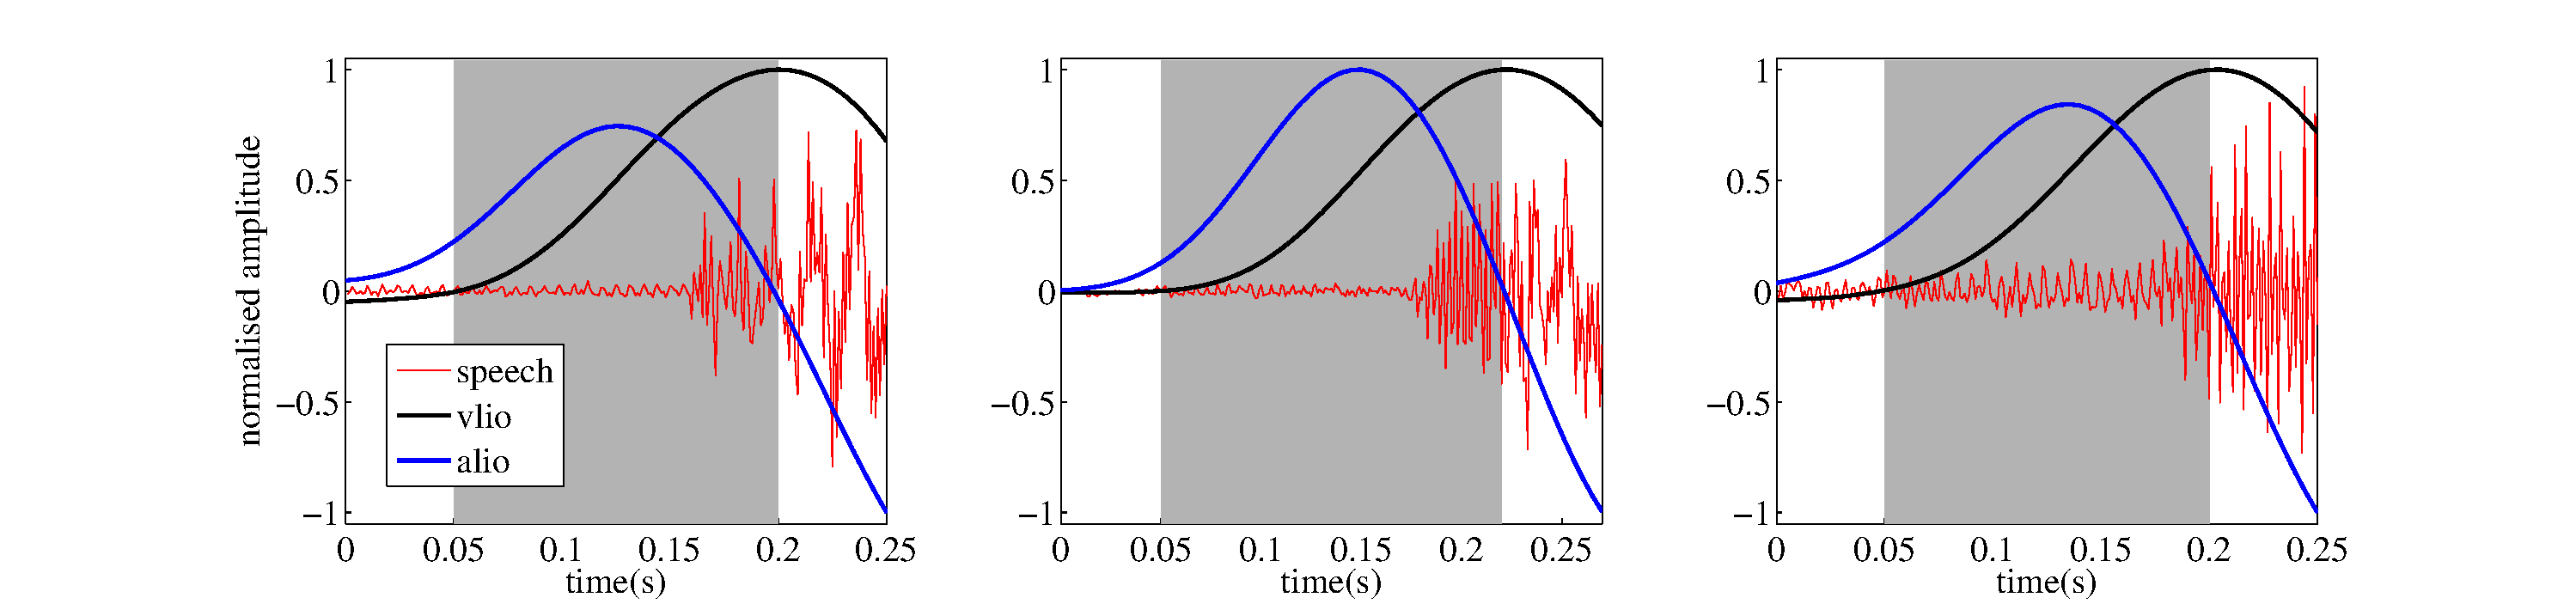
\includegraphics[width=\textwidth]{figs/samples}}
  \caption{The speech signal and motor trajectories of lips opening
    velocity (\vlio) and acceleration (\alio) during utterances containing /b/.
    Left to right: /ba/, subject $5$; /ba/, subject $2$; and /bufalo/, subject $5$.
    The gray zone denotes the detected start and ending of the plosion. All signals
    are normalised over the indicated time frame, for visualisation purposes.}
  \label{fig:isdView}
\end{figure*}

\begin{figure*}[t]
  \centerline{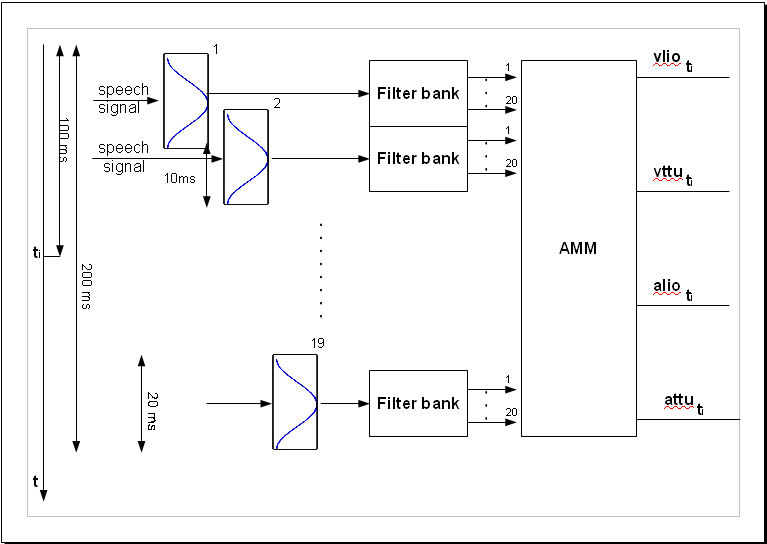
\includegraphics[width=\textwidth]{figs/audio2motor}}
  \caption{From speech signal to reconstructed motor information. To reconstruct
    a single sample of \vlio, \alio, \vttu\ and \attu\ at time $t_i$ the
    spectrogram of nineteen $20$-millisecond long Hamming windows is evaluated.
    One window is centered at time $t_i$, $9$ windows precede it
    and $9$ windows follow it. Each window overlaps by $10$ milliseconds
    with the preceding window. The spectrogram is computed by using a
    $20$-filter Mel-scale filterbank.}
  \label{fig:amm}
\end{figure*}

\begin{figure*}[t]
  \centerline{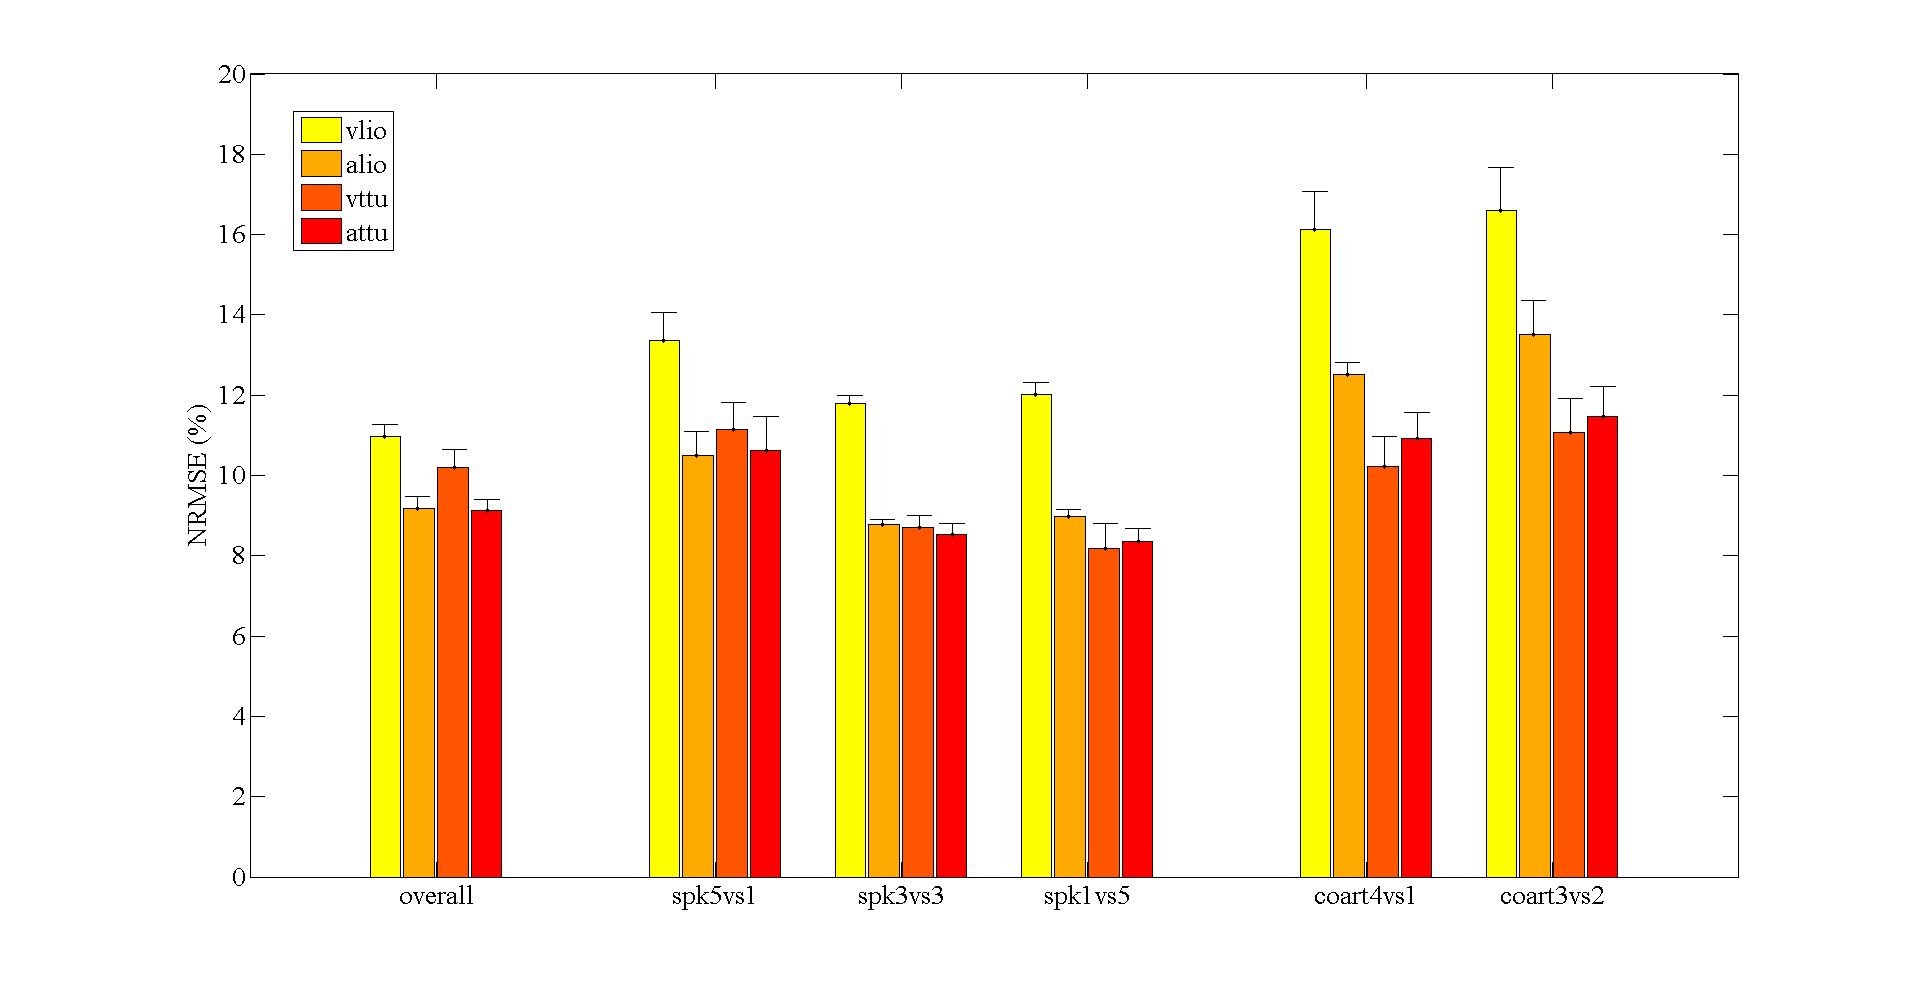
\includegraphics[width=\textwidth]{figs/AMM}}
  \caption{Quantitative performance of the AMM. For each cross-validation schema (overall, etc.)
    and output signal (\vlio, etc.) the NRMSE average value and standard error of the mean
    are reported.}
  \label{fig:amm_perf}
\end{figure*}

\begin{figure*}[t]
  \centerline{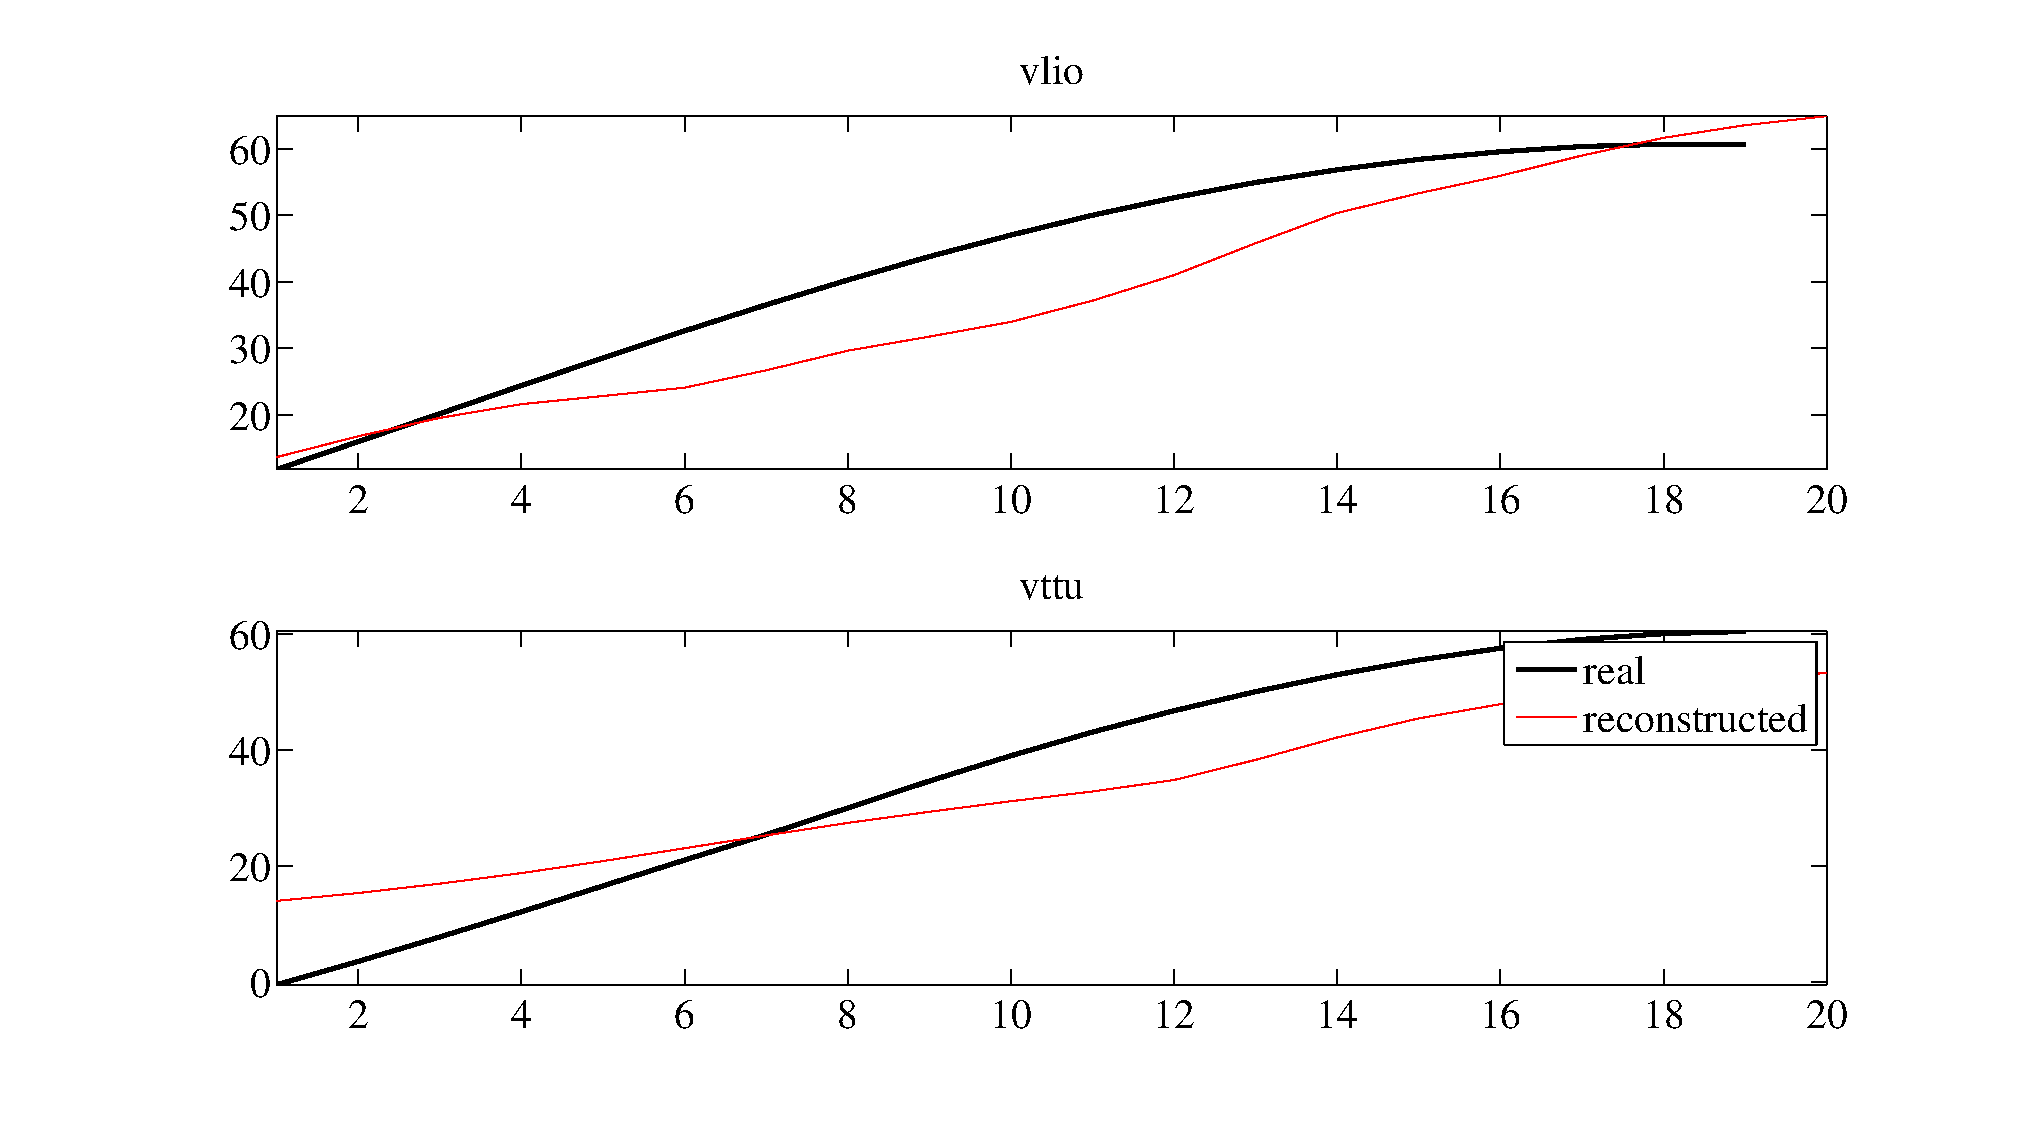
\includegraphics[width=\textwidth]{figs/recMIs}}
  \caption{Real and AMM-reconstructed \vlio\ and \vttu\ for subject $6$ uttering
    the /t/ in \emph{accento?} (accent). Notice the apparent gap in the quality
    of the reconstruction, favouring in this case the labiodental trajectory (\vttu).}
  \label{fig:example}
\end{figure*}

\begin{figure*}[t]
  \centerline{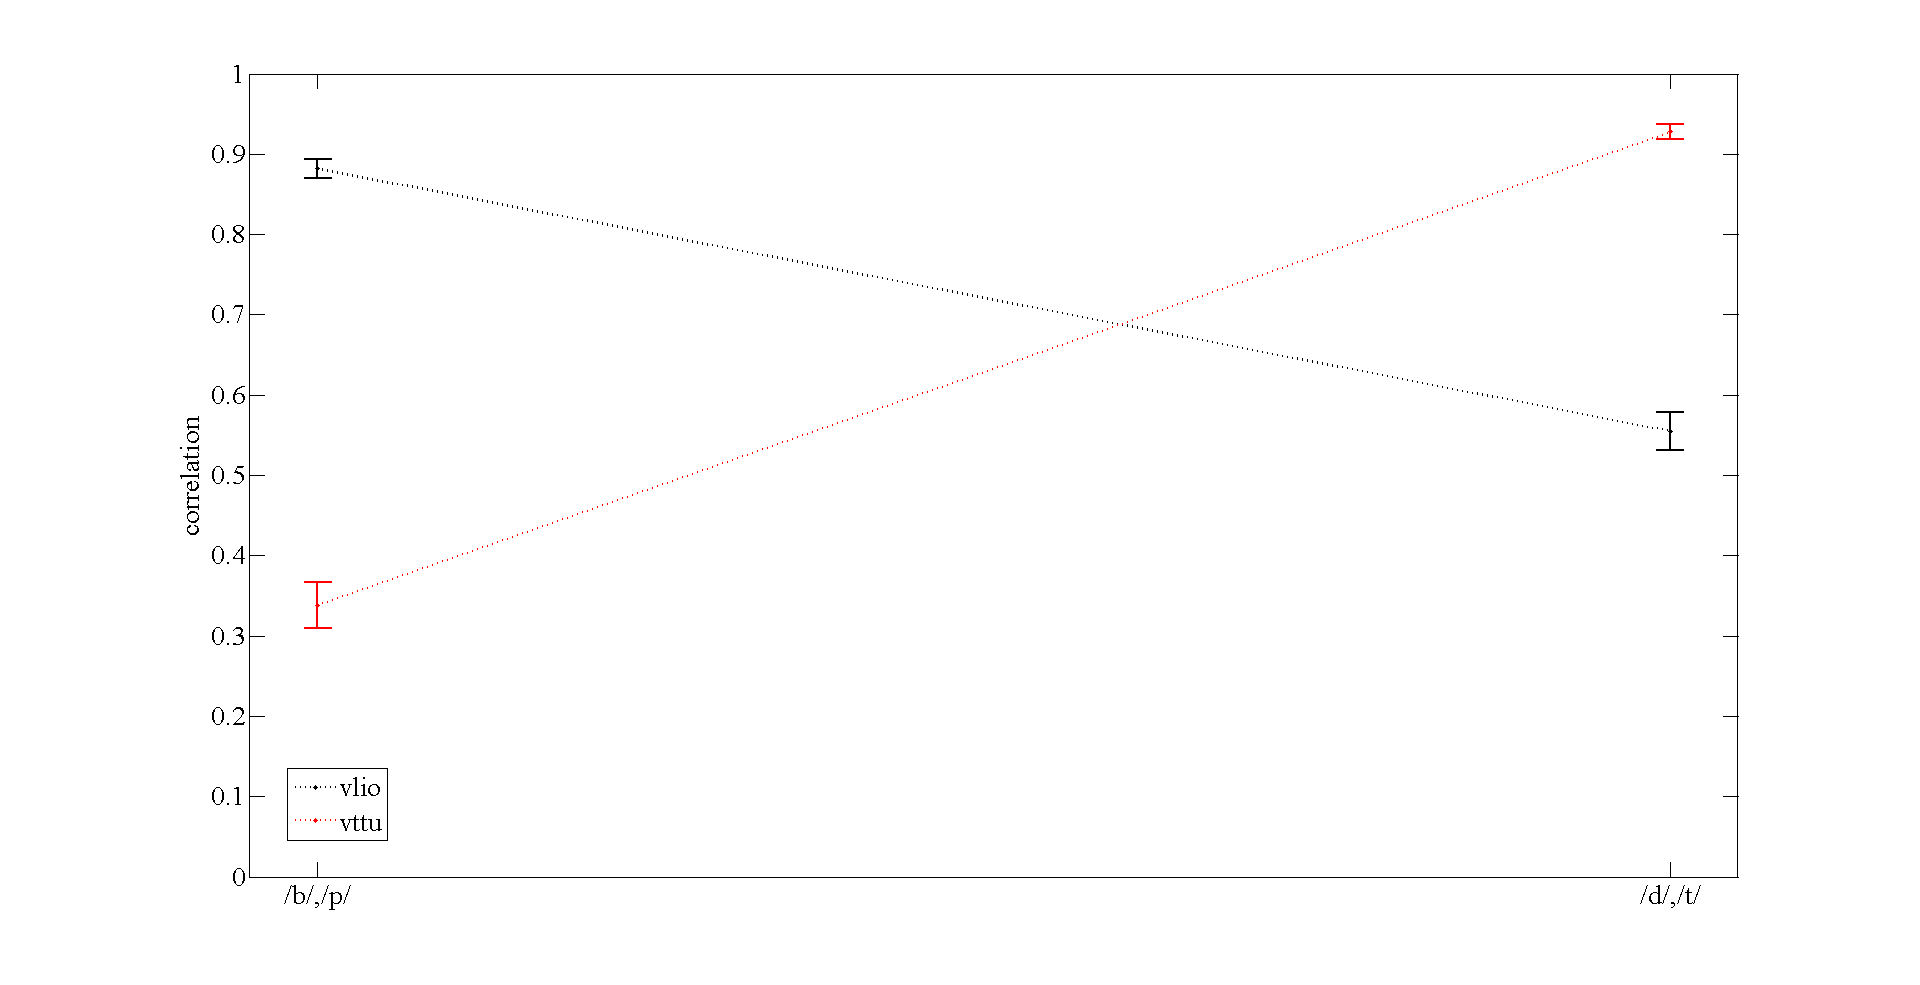
\includegraphics[width=\textwidth]{figs/doubleDiss}}
  \caption{Double dissociation of correlation between real and AMM-reconstructed MI
    (mean and standard error of the mean). Mean coefficients are significantly
    higher for \vlio\ when ``listening'' to labials than dentals and vice-versa.
    The \overall\ CV schema is used.}
  \label{fig:DD}
\end{figure*}

\begin{figure*}[t]
  \centerline{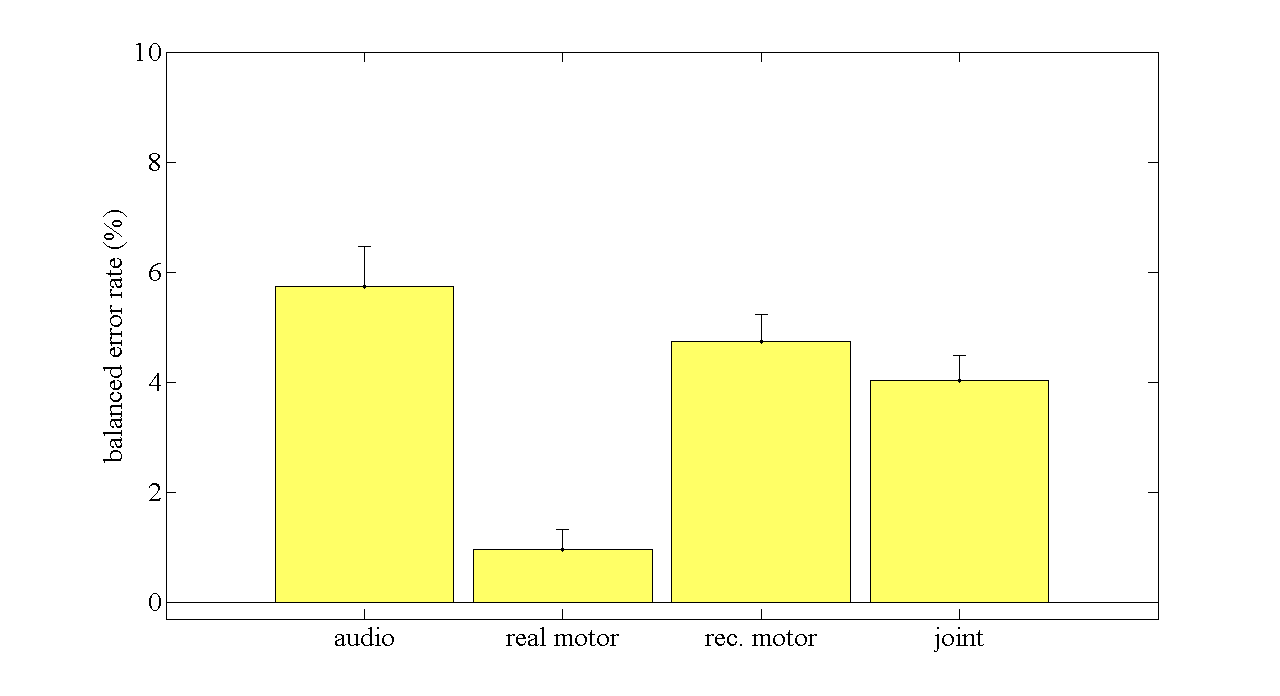
\includegraphics[width=\textwidth]{figs/exp1}}
  \caption{Balanced error rate in classification of bilabials and dentals obtained
    in the \overall\ CV schema, using audio features, real motor features,
    motor features reconstructed by the AMM, and by joining the audio and
    reconstructed-motor models.}
  \label{fig:class1_perf}
\end{figure*}

\begin{figure*}[t]
  \centerline{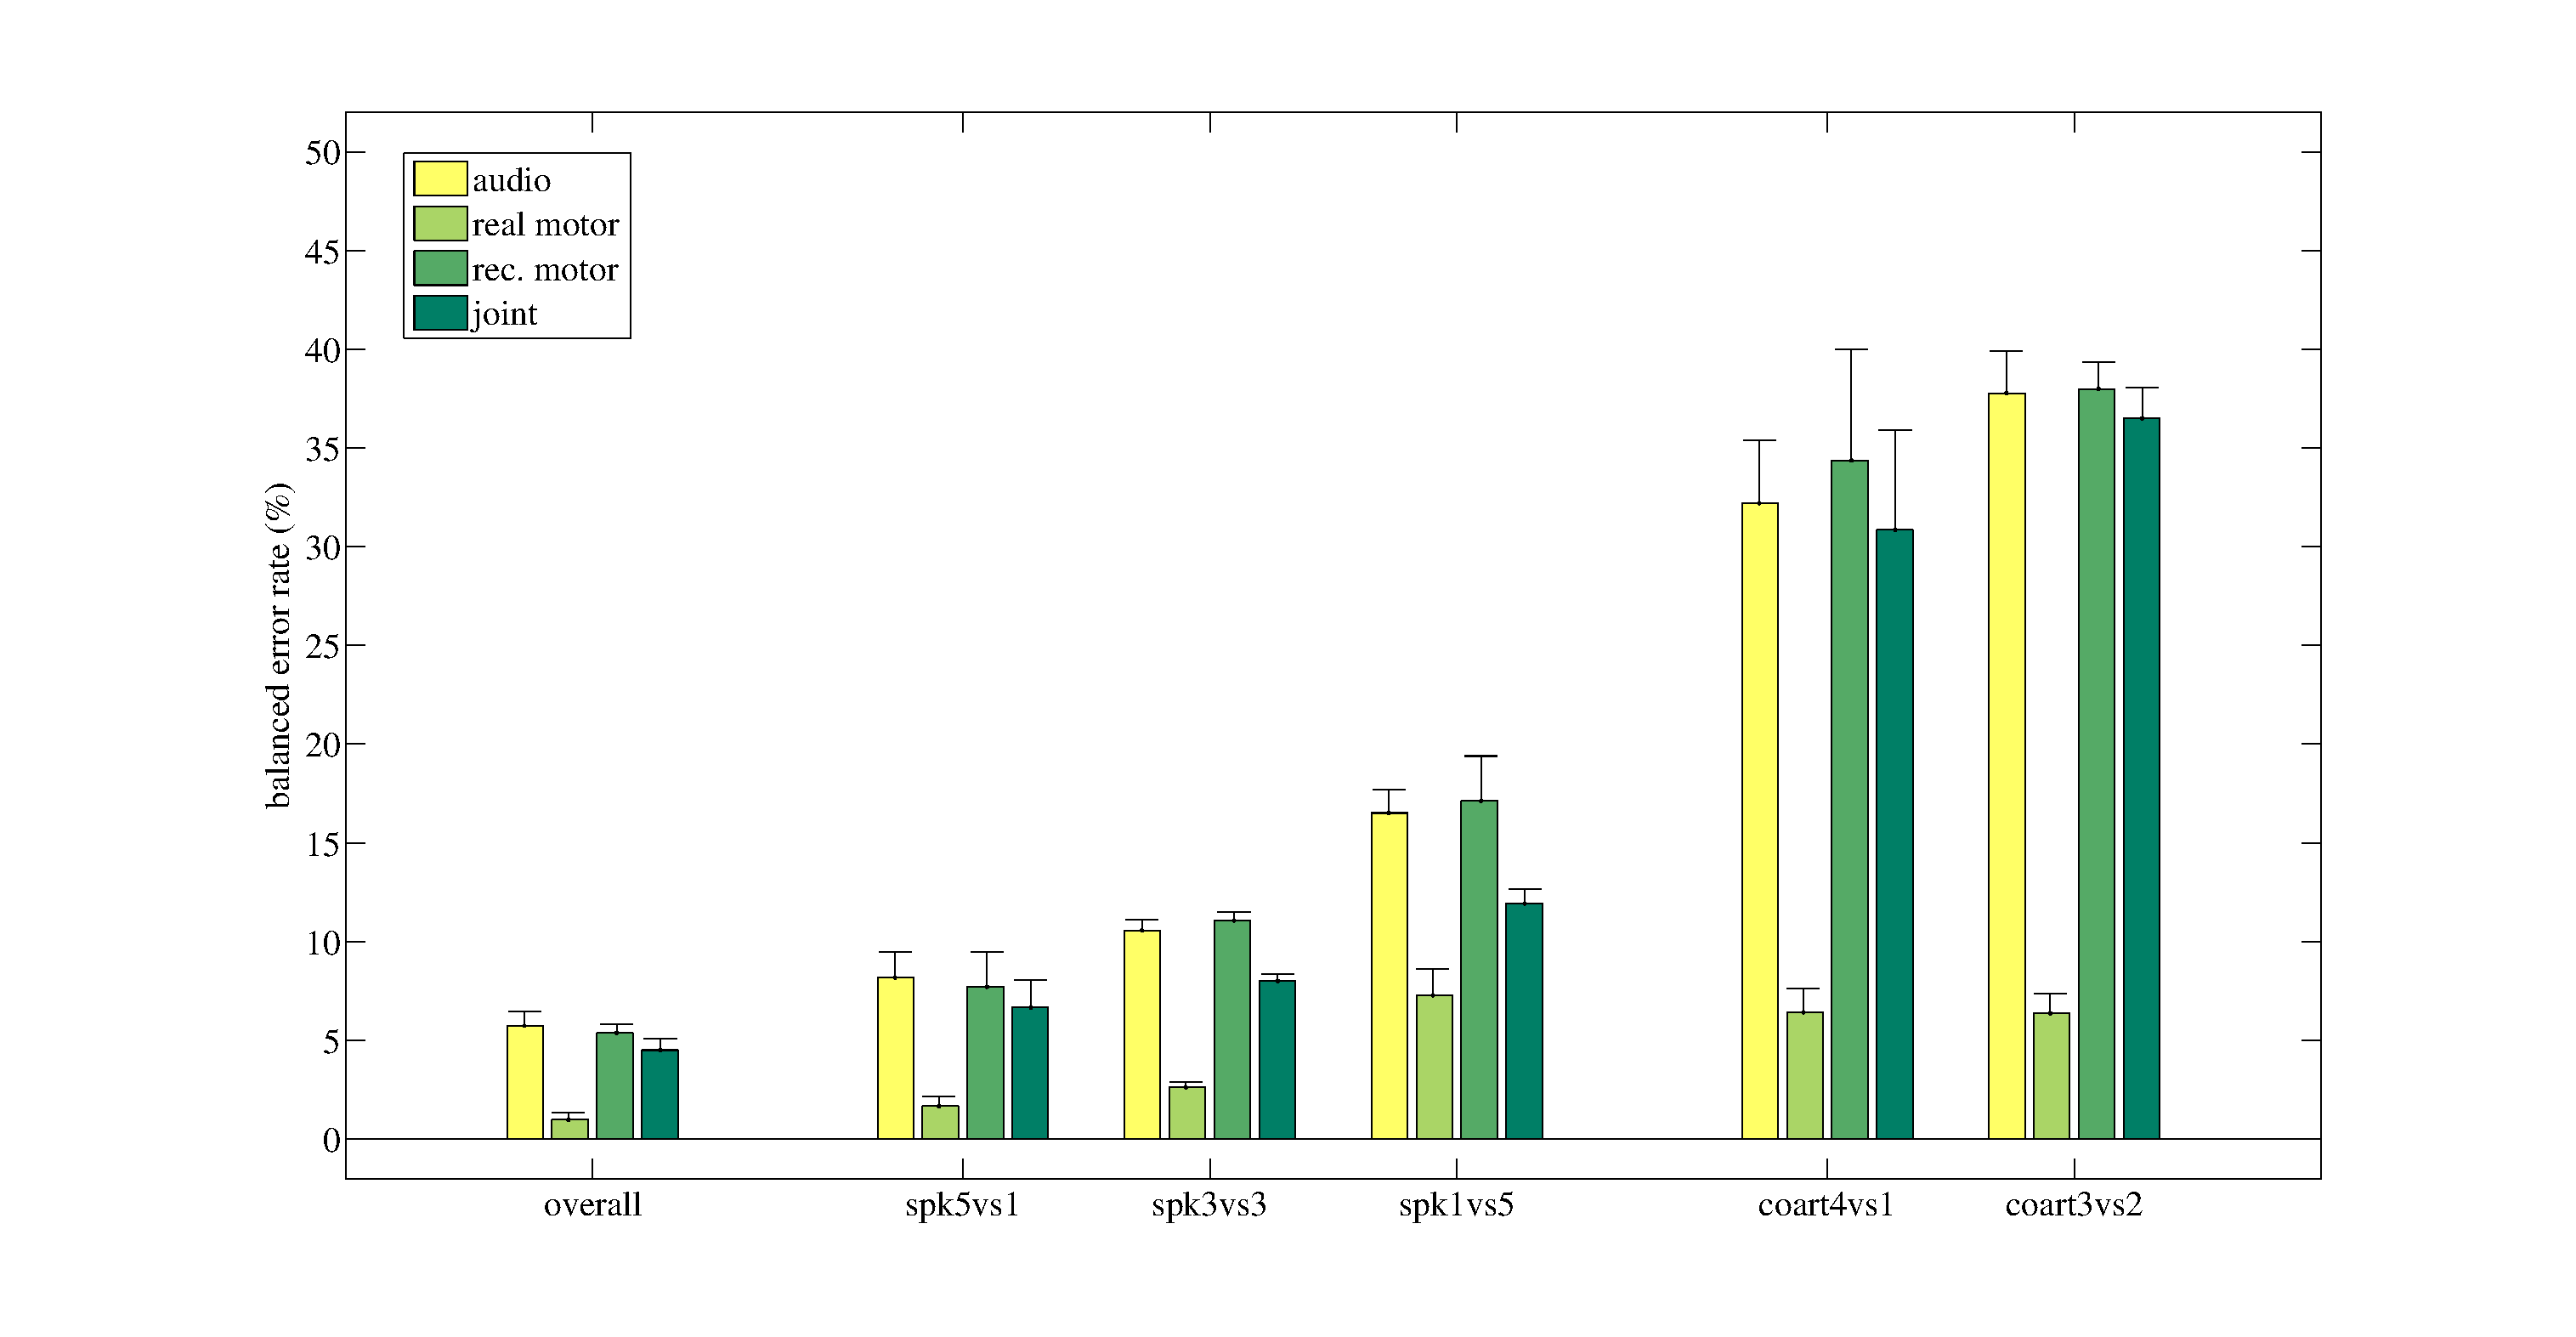
\includegraphics[width=\textwidth]{figs/exp2}}
  \caption{Balanced error rate in classification of bilabials and dentals for each
    CV schema, using the four sets of features of Figure \ref{fig:class1_perf}.}
  \label{fig:class2_perf}
\end{figure*}

\begin{figure*}[t]
  \centerline{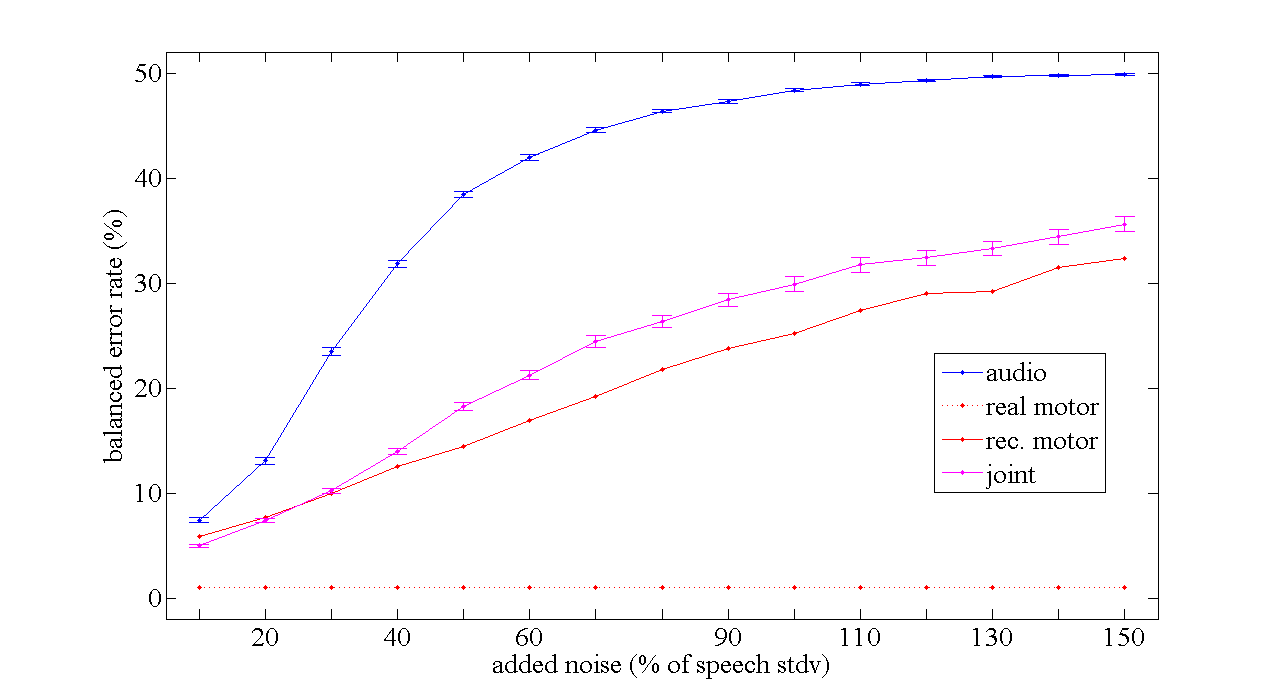
\includegraphics[width=\textwidth]{figs/exp3}}
  \caption{Balanced error rate in classification of bilabials and dentals for the
    \overall\ CV schema as noise is added, using the sets of features of Figure
    \ref{fig:class1_perf}.}
  \label{fig:class3_perf}
\end{figure*}

\end{document}
